\documentclass{standalone}
\usepackage{xparse}
\usepackage[dvipsnames]{xcolor}
\usepackage{tikz}
\usepackage{pgfbaseshapes}
\usetikzlibrary{arrows,automata,positioning,matrix,decorations.pathreplacing,fit,shapes.geometric,calc}
\pgfdeclarelayer{background1}
\pgfdeclarelayer{background2}
\pgfdeclarelayer{background3}
\pgfdeclarelayer{foreground1}
\pgfdeclarelayer{foreground2}
\pgfdeclarelayer{foreground3}
\pgfdeclarelayer{middleground1}
\pgfdeclarelayer{middleground2}
\pgfdeclarelayer{middleground3}
\pgfsetlayers{background1,background2,background3,middleground1,middleground2,middleground3,main,foreground1,foreground2,foreground3}
\tikzstyle{var}=[circle,draw,fill=white,inner sep=0pt,minimum size=25pt]
\tikzstyle{edge}=[->,>=stealth]
\tikzstyle{subtree}=[draw=none,fill=black!10]
\tikzstyle{subtreelinebase}=[line width=1pt]
\tikzstyle{subtreeline}=[subtreelinebase,densely dotted]
\tikzstyle{subtreeedge}=[subtreelinebase,edge,shorten >=12.5pt,shorten <=12.5pt]
\newcommand*{\xy}[2]{{#1+(#2-#1)/2},{(#2-#1)/2}}
\NewDocumentCommand{\subtree}{ m m O{_} O{} O{} O{0pt} O{1} }{
  \pgfmathsetmacro{\lpone}{int(#1+1)}
  \pgfmathsetmacro{\rmone}{int(#2-1)}
  \node[var] (_) at (\xy{#1}{#2}) {$x_{#1:#2}$};
  \begin{pgfonlayer}{background#7}
    \path[subtree,#5] ($(x#1_\lpone.center)+#6$) -- ($(_.center)+#6$) -- ($(x\rmone_#2.center)+#6$);
  \end{pgfonlayer}
  \begin{pgfonlayer}{background#7}
    \path[subtreeline,#4] ($(x#1_\lpone.center)+#6$) -- ($(_.center)+#6$) -- ($(x\rmone_#2.center)+#6$);
  \end{pgfonlayer}
  \begin{pgfonlayer}{foreground#7}
    \draw[subtreeedge,#4] ($(#3)+#6$) -- ($(_)+#6$);
  \end{pgfonlayer}
}
\NewDocumentCommand{\split}{ m m m O{_} O{} O{0pt} O{1} O{1} }{
  \subtree{#1}{#2}[#4][draw=#5][fill=#5!10,opacity=0.7][(#6,-#6)][#7]
  \subtree{#2}{#3}[#4][draw=#5][fill=#5!10,opacity=0.7][(#6,#6)][#8]
}
\newcommand*{\term}[1]{
  \pgfmathsetmacro{\kmone}{int(#1-1)}
  \pgfmathsetmacro{\kpone}{int(#1+1)}
  \node[var] (y#1) at ($(\xy{#1}{\kpone})-(0,1)$) {$y_{\kpone}$};
  \node[var] (x#1_\kpone) at (\xy{#1}{\kpone}) {$x_{#1:\kpone}$};
  \draw[edge] (x#1_\kpone) -- (y#1);
}
\begin{document}
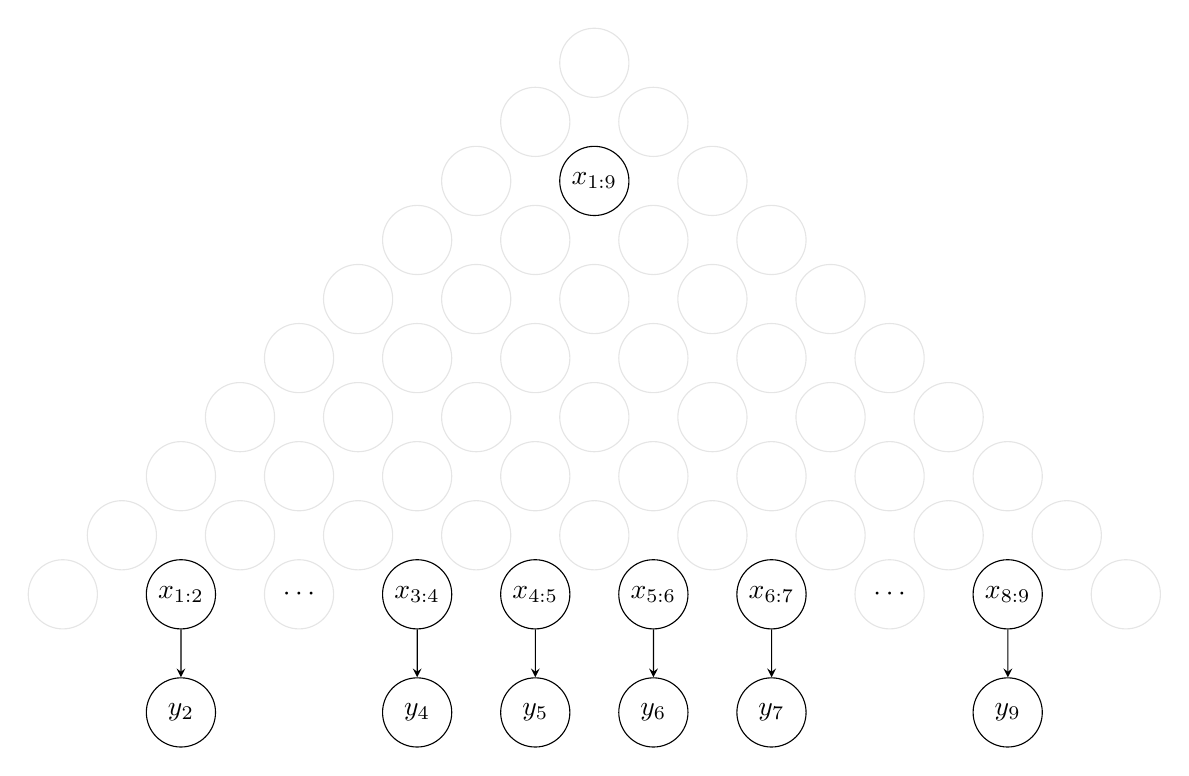
\begin{tikzpicture}[scale=1.5]
  \def\n{10}
  \pgfmathsetmacro{\nmone}{int(\n-1)}
  % full grid
  \def\offset{1}
  \foreach \stop in {\offset,...,\n} {
    \pgfmathsetmacro{\stopminusoffset}{int(\stop-\offset)}
    \foreach \start in {0,...,\stopminusoffset} {
      \begin{pgfonlayer}{background1}
        \node[var,draw=black!10] at (\xy{\start}{\stop}) {};
      \end{pgfonlayer}
    }
  }
  % bottom row
  % \foreach \k in {0,...,\nmone} {
  \foreach \k in {1,3,4,5,6,8} {
    \term{\k}
  }
  \node at (\xy{2}{3}) {$\cdots$};
  \node at (\xy{7}{8}) {$\cdots$};
  % individual nodes
  \def\start{1}
  \def\stop{9}
  % \node[var] at (\xy{0}{\n}) {$x_{0:\n}$};
  \node[var] (par) at (\xy{\start}{\stop}) {$x_{\start:\stop}$};

  \split{\start}{4}{\stop}[par][BurntOrange][0.7mm][3][1]
  \split{\start}{5}{\stop}[par][RoyalBlue][0mm][2][2]
  \split{\start}{6}{\stop}[par][OliveGreen][-0.7mm][1][3]
\end{tikzpicture}
\end{document}

%%% Local Variables:
%%% mode: latex
%%% TeX-master: t
%%% End:
